\section{Transmission frequency reconfiguration}

\npar The sequence diagram of this scenario is splitted in two parts for the
sake of clarity. The first part is an overview and the second diagram
contains a detailed diagram of the remote module communication unit.

\begin{figure}[H]
	\begin{centering}
		% TODO Figure
		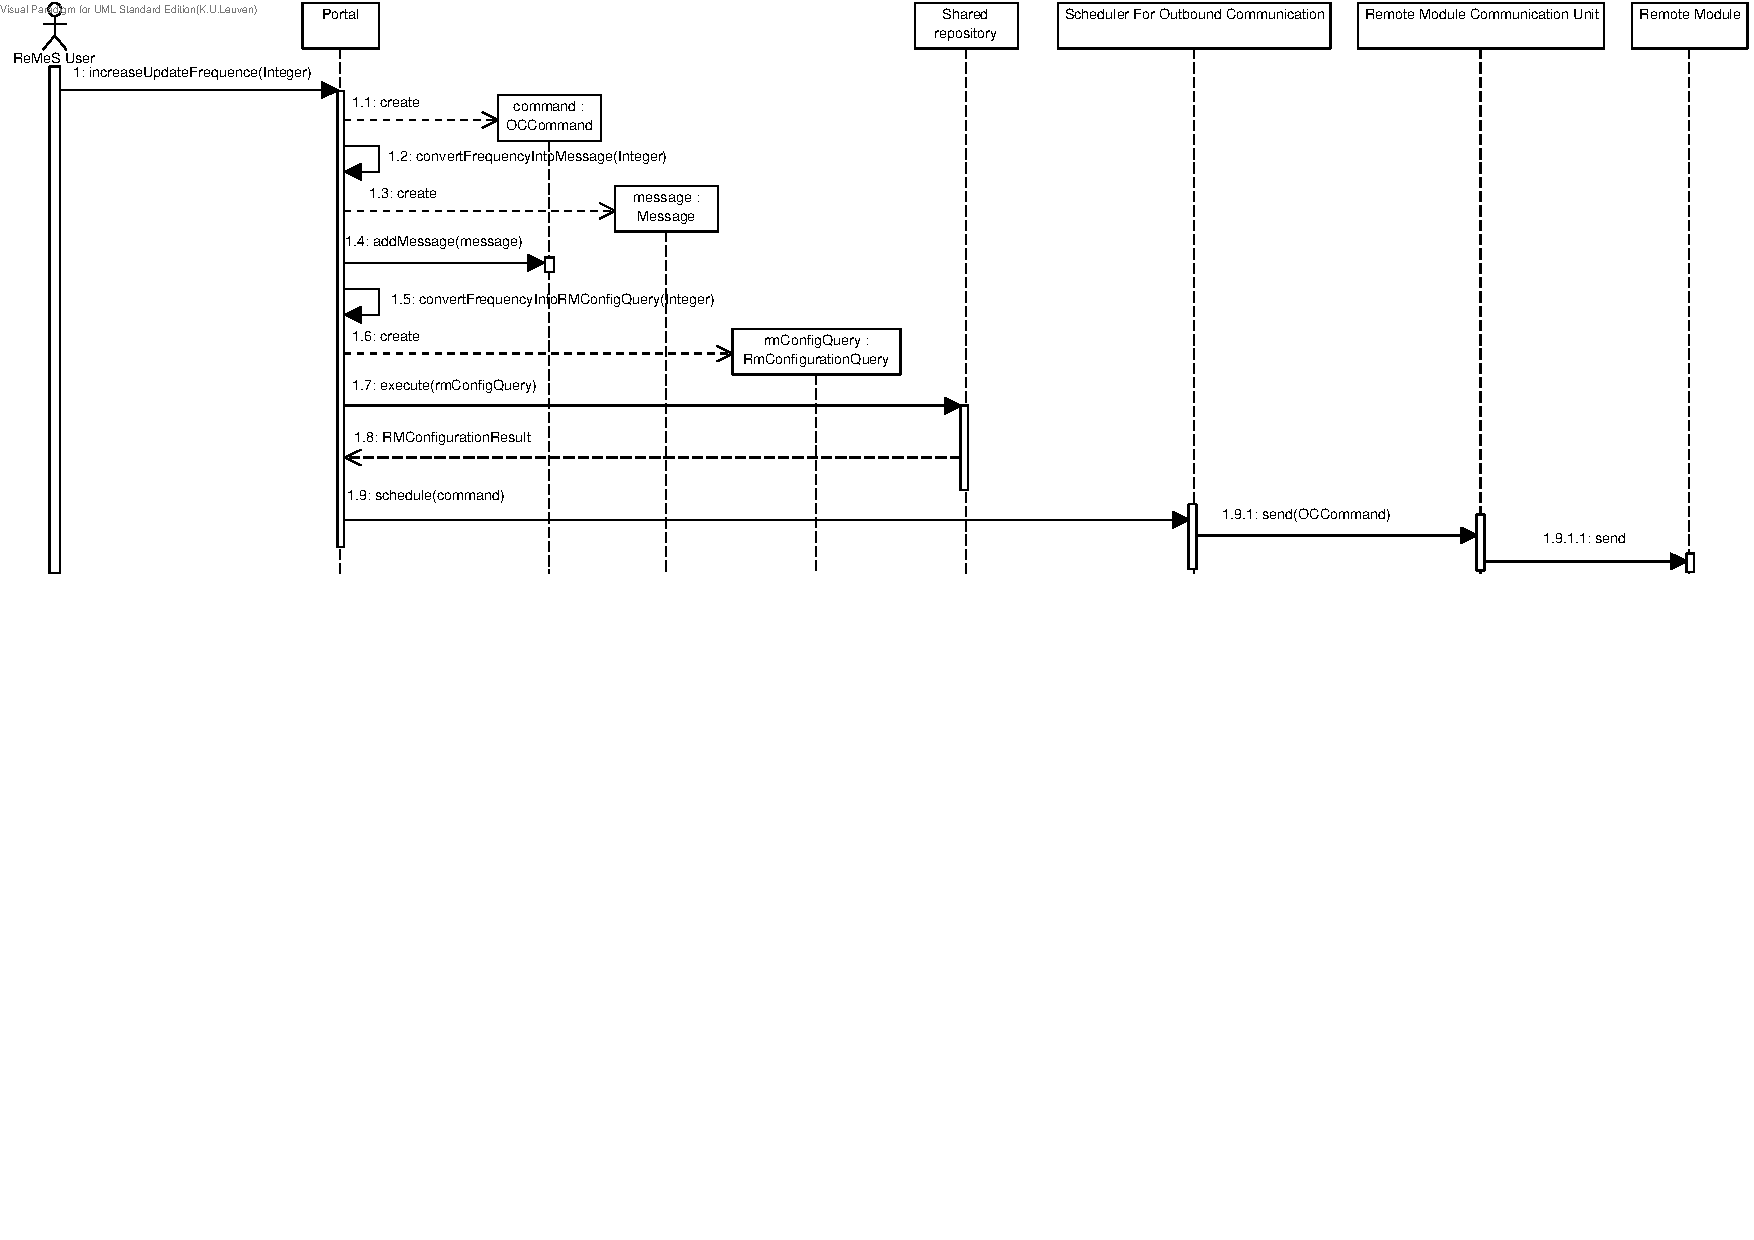
\includegraphics[width=1.4\textwidth,angle=90]{figs/scenario-5-3-2.pdf}
		\caption{The sequence diagram of scenario: Transmission frequency reconfiguration.}
		\label{fig:scenario-5-3-2}
	\end{centering}
\end{figure}

\npar In step 1.6, the drafted query is a store query for the new transmission
frequency. 

\begin{figure}[H]
	\begin{centering}
		% TODO Figure
		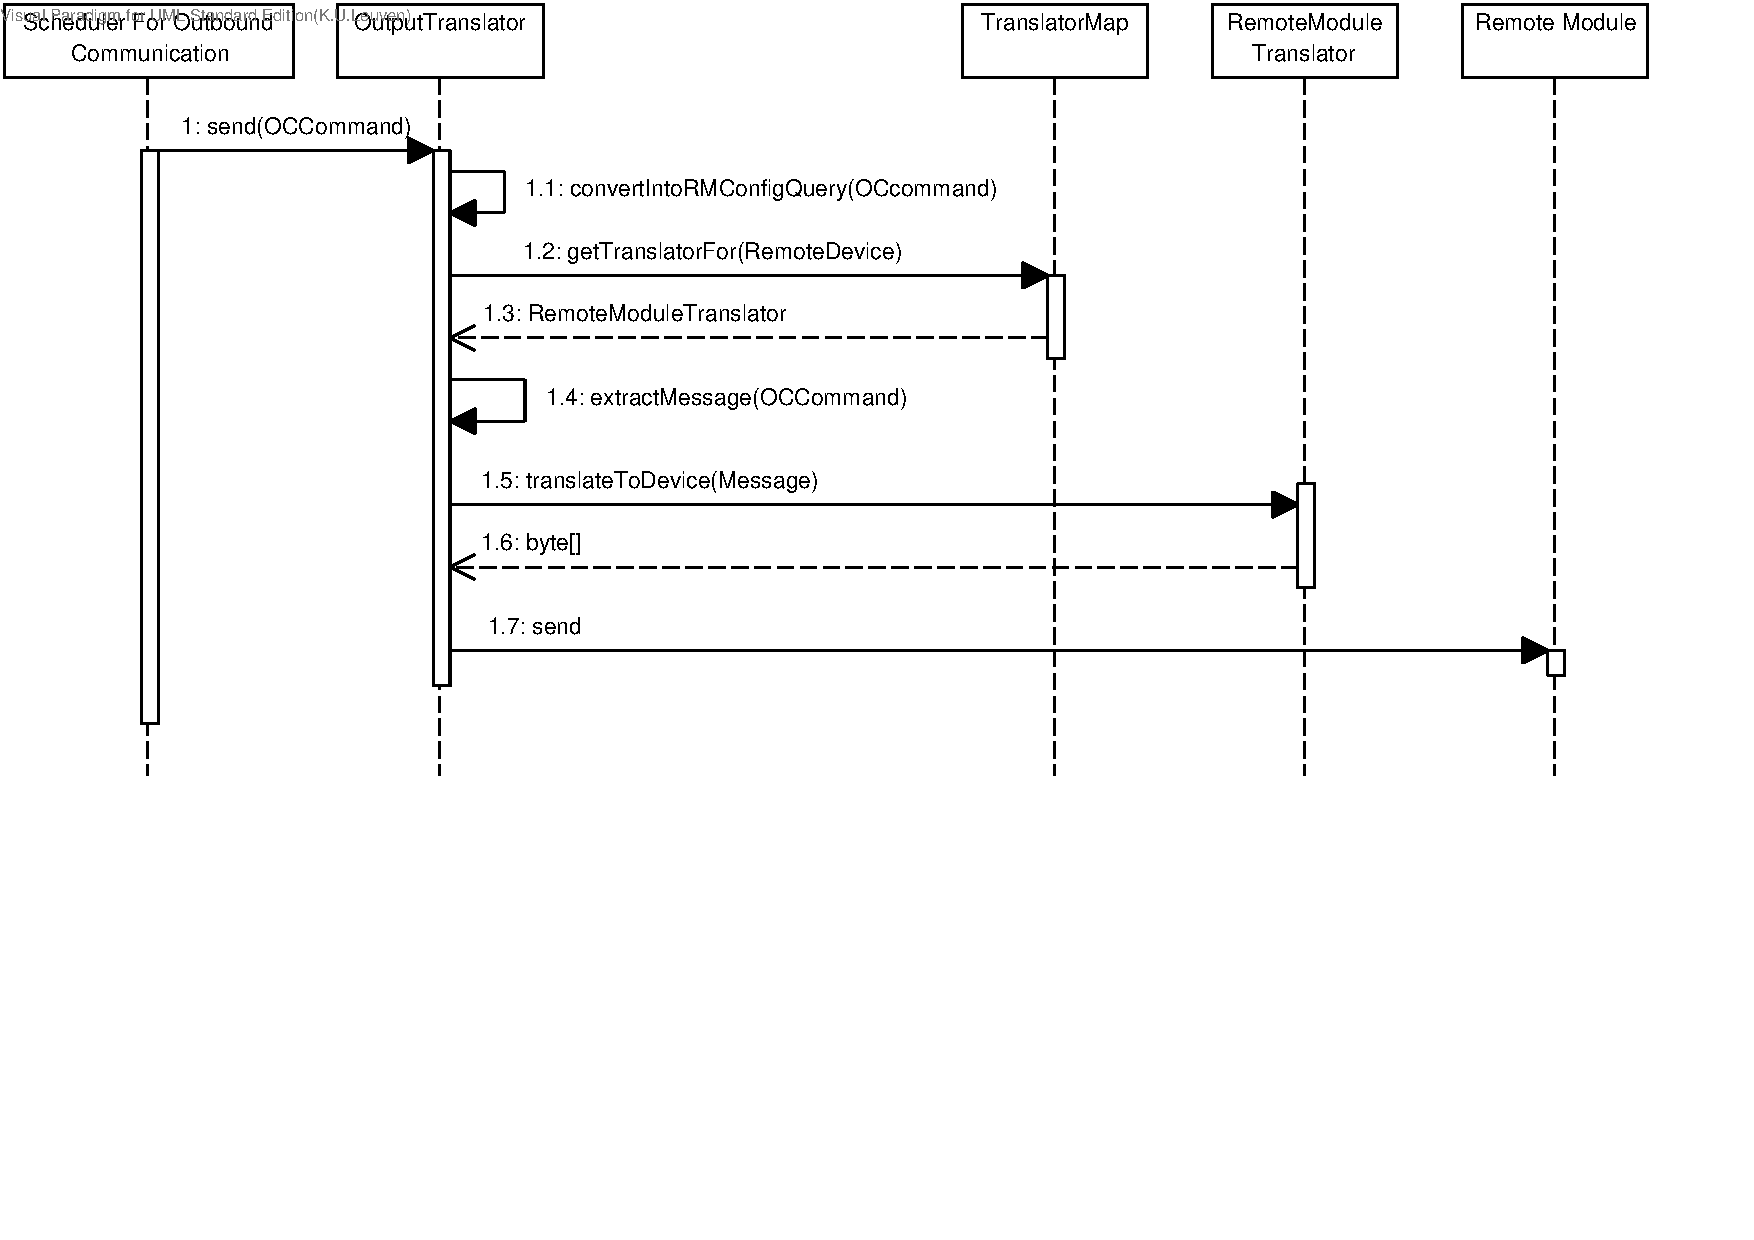
\includegraphics[width=\textwidth]{figs/scenario-5-3-2a.pdf}
		\caption{The sequence diagram of the remote module communication unit}
		\label{fig:scenario-5-3-2a}
	\end{centering}
\end{figure}

\npar The physical communication towards the remote module is modelled as a
``send'' message in the last step of diagram \ref{fig:scenario-5-3-2a}.
